This layer is the integration of the UI and camera in details.

\begin{figure}[h!]
	\centering
 	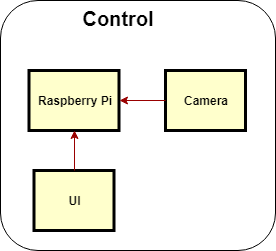
\includegraphics[width=0.60\textwidth]{images/Control_Layer}
 \caption{Control layer diagram}
\end{figure}

\subsection{User Interface (UI)}
The user interface operates through a browser that allow the user to give specifics task to the UR5. User interaction is via a monitor and mouse attached to the Raspberry Pi.

\subsubsection{Assumptions}
The browser the user will be using is Google Chrome. Other browser may work just as well. This project, however, tested and developed the UI through Google Chrome.

\subsubsection{Responsibilities}
The purpose of this UI is to allow the user to gives specific command to the UR5. The commands are as follows:
\newline Home  		: Move UR5 to default position.
\newline Start 		: Make grill cheese sandwich.
\newline Stop  		: Cease function.
\newline Rack Tool 	: Put away tool.
\newline Grab Tool 	: Grab tool.
	
*The tool for this project specifically is a spatula. Other tools will be implement later in the future.

\subsubsection{Subsystem Interfaces}
The UI connects to the Raspberry Pi.

\begin {table}[H]
\caption {UI interfaces} 
\begin{center}
    \begin{tabular}{ | p{1cm} | p{6cm} | p{3cm} | p{3cm} |}
    \hline
    ID & Description & Inputs & Outputs \\ \hline
    \#1 & Raspberry Pi & \pbox{3cm}{N/A} & \pbox{3cm}{UI Commands (via mouse)}  \\ \hline
    \end{tabular}
\end{center}
\end{table}

\subsection{Camera}
The camera use to determine the location of certain object(sandwich) or if there is another object in the way of the UR5.

\subsubsection{Assumptions}
The camera is a 720p or higher.
At least one camera.

\subsubsection{Responsibilities}
The purpose of the camera is to determine the location of the sandwich relative to its position so that the UR5 can pick up the sandwich. Its other responsibility is also to detect foreign obstacle or human being so that it can stop before colliding.

\subsubsection{Subsystem Interfaces}
The camera connects to the Raspberry Pi.

\begin {table}[H]
\caption {Camera interfaces} 
\begin{center}
    \begin{tabular}{ | p{1cm} | p{6cm} | p{3cm} | p{3cm} |}
    \hline
    ID & Description & Inputs & Outputs \\ \hline
    \#1 & Raspberry Pi & \pbox{3cm}{N/A} & \pbox{3cm}{Location of sandwich\\ Detect foreign obstacle or human being}  \\ \hline
    \end{tabular}
\end{center}
\end{table}

\subsection{Raspberry Pi}
The Raspberry Pi houses all of the programs produced in this project.  It generates the UI via a node.js server for the user to interact with and output robot commands to the network system based on user input.
\subsubsection{Assumptions}
That all hardware connections are supported and configured properly: mouse and monitor are set up, and network connection to the UR5 is established.
\subsubsection{Responsibilities}
To handle all inputs from the user and outputs to the network.
\subsubsection{Subsystem Interfaces}

\begin {table}[H]
\caption {Raspberry Pi interfaces} 
\begin{center}
    \begin{tabular}{ | p{1cm} | p{6cm} | p{3cm} | p{3cm} |}
    \hline
    ID & Description & Inputs & Outputs \\ \hline
    \#1 & UI & \pbox{3cm}{UI Commands} & \pbox{3cm}{N/A}  \\ \hline
    \#2 & Camera & \pbox{3cm}{Location of sandwich\\ Detect foreign obstacle or human being} & \pbox{3cm}{N/A}  \\ \hline
    \end{tabular}
\end{center}
\end{table}

